\section{Les LLNs}

% \begin{frame}{Architecture réseau}
%   \begin{figure}
%     \centering
%     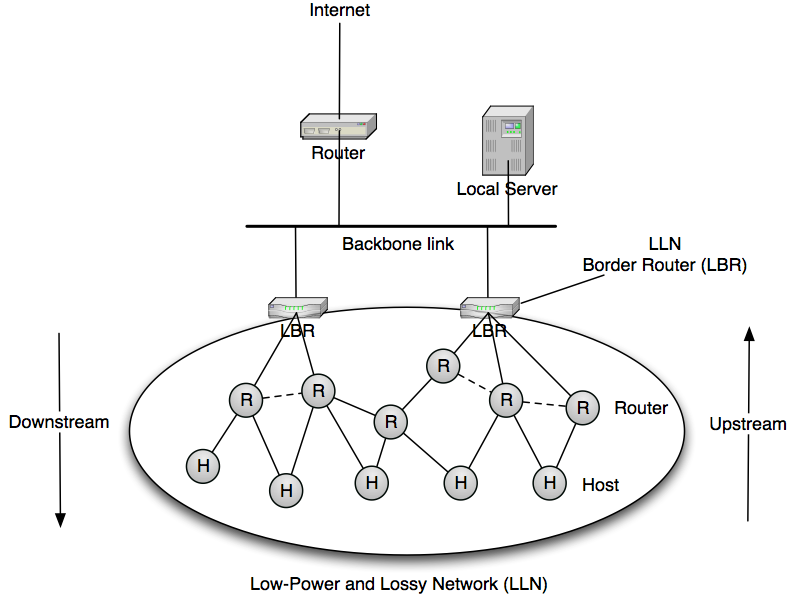
\includegraphics[scale=.3]{figures/rpl.png}
%   \end{figure}
%   \pnote{
%     Il est à noter que les routeurs peuvent aussi héberger des serveurs applicatifs
%   }
% \end{frame}

\begin{frame}{Architecture d'un nœud}
  \begin{figure}
    \centering
    \begin{tikzpicture}[->,>=latex,shorten >=1pt, thick,main node/.style={fill=blue!20,draw}, scale = .8, every node/.style={scale = .8}]

  \node[main node] (cpu) {\begin{tabular}{c}Micro-contrôleur\end{tabular}};
  % \node[main node, below=of cpu] (battery) {\begin{tabular}{c}Source d'énergie\end{tabular}};
  \node[main node, above=of cpu] (radio) {\begin{tabular}{c}Radio\end{tabular}};
  \node[main node, right=of cpu] (memoire) {\begin{tabular}{c}Mémoire\end{tabular}};
  \node[main node, left=of cpu] (convert) {\begin{tabular}{c}Convertisseurs\\ analogique / numérique \end{tabular}};

  % \node[main node, below=of convert] (actionneur) {\begin{tabular}{c}Actionneur\end{tabular}};
  \node[main node, above=of convert] (sensor) {\begin{tabular}{c}Capteur / Actionneur\end{tabular}};

  \path
       % (actionneur) edge[<-] (convert.south) 
       (sensor) edge[->] (convert.north) 
       (convert) edge[<->] (cpu) 
       (cpu)  edge[<->] (radio)
       (cpu) edge[<->] (memoire)
  ;

\end{tikzpicture}

  \end{figure}
  \begin{block}{Contraintes et solutions}
    \begin{itemize}
      \item Faibles ressources matérielles (Processeur, mémoire, stockage) $\to$ Système d'exploitation et applications adaptés.
      \item Réserve d'énergie limitée $\to$ Cycle de sommeil.
    \end{itemize}
  \end{block}
  \pnote{
    OpenMote Proc 32 MHz, 32 Kbytes of RAM and 512 Kbytes of Flash,
  }
  \pnote{
    Portée de quelques dizaines de mètres à plusieurs kilomètres selon les technologies
  }
  \pnote{
    - L'hétérogéneité provient de la profusion des acteurs et du faible cout d'entrée dans les marchés
  }
  \pnote{
  Composants variés et généralement peu onéreux.
    - Dire que les progrès technologiques visent à rendre les composants moins chers au lieu de performants
  }
  \pnote{
    Modèle de programmation qui évite les allocations mémoire
  }
  \pnote{
    On peut mentionner aussi l'énergy harvesting
  }
  \pnote{
    - Faible puissance d'émission
  }
  \pnote{
    - Liens assez mauvais et bruité
  }
  \pnote{
    - Mentionner les problèmes de multi-path fading
  }
\end{frame}

\begin{frame}{Consommation de la radio}

  \begin{block}{Exemple: TmoteSky - CC2420 - ContikiMAC}
    \begin{itemize}
      % \item Trame de taille maximale (127 octets)
      \item Écoute: 63 mW, Transmission: 60mW
      \item CPU: 5mW (Actif) / 0.1mW (Sommeil)
    \end{itemize}
  \end{block}

  \begin{figure}
    \centering
    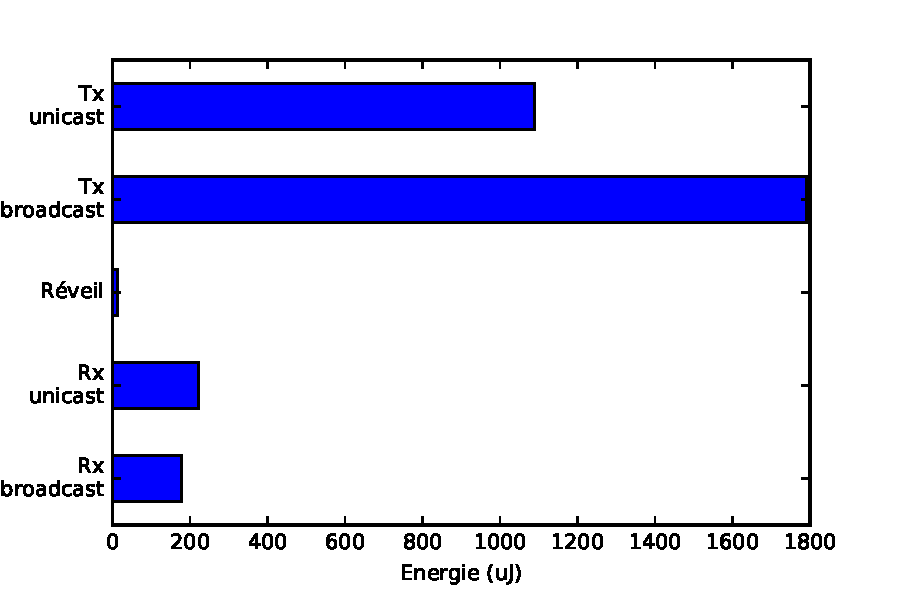
\includegraphics[width=0.6\textwidth]{figures/consommation_contikimac.pdf}
  \end{figure}

  Objectif: Minimiser l'utilisation de la radio.
\end{frame}

\DeclarePairedDelimiter{\ceil}{\lceil}{\rceil}

\definecolor{mycolor}{RGB}{141,177,227}
\newcommand{\mycbox}[1]{\tikz{\path[draw=mycolor,fill=mycolor] (0,0) rectangle (.3cm,.3cm);}}

\begin{frame}{Strobing (MAC asynchrone)}
  % \begin{block}{\ieee{}}
  %   $T_p = \frac{\mathcal{L}(f)}{R} \ceil[\Big]{\frac{\mathcal{L}(p)}{L}}$
  % \end{block}

  \begin{figure}[ht]
    \centering
    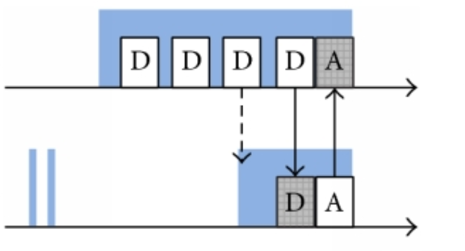
\includegraphics[width=.6\textwidth]{figures/contikimac.png}
  \end{figure}
  \begin{block}{Légende}
    \begin{description}
      \item[D] Trame de données
      \item[A] Trame d'acquittement
      \item[\mycbox{blue}] Radio activée
    \end{description}
  \end{block}
  \begin{alertblock}{Point clé}
    \begin{itemize}
      \item Différence entre paquet logique et trame physique
    \end{itemize}
  \end{alertblock}
  \pnote{
    - En blue: La fenetre de réception
  }
  \pnote{
    - blanc: Trame de données/ack transmises mais non reçue
  }
  \pnote{
    - noir: Trame de données/ack transmis et reçue
  }
  \pnote{
    $T_\detect$ est le temps que le transmetteur va passer en écoute juste après une tentative de transmission pour détecter son éventuel succès par un acquittement d'un récepteur juste après l'envoi d'une trame de donnée.
  }
  \pnote{
    ti: the interval between each packet transmission. (0.4 ms)
  }
  \pnote{
    tr: the time required for a stable RSSI, needed for a stable CCA indication.
  }
  \pnote{
    tc: the interval between each CCA.
  }
  \pnote{
    ta: the time between receiving a packet and sending the acknowledgment packet.
  }
  \pnote{
    td: the time required for successfully detecting an acknowledgment from the receiver. (0.16 ms)
  }
  \pnote{
    ts, the transmission time of the shortest packet, must be larger than tr + tc + tr (0.884 ms)
  }
\end{frame}


\begin{frame}{Architecture générale d'un réseau de capteurs}
  \begin{figure}
    \centering
    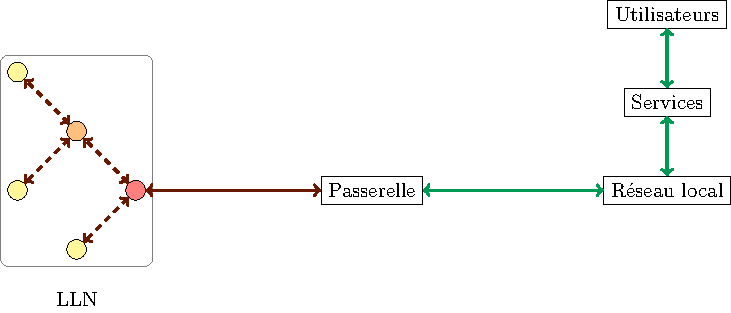
\includegraphics[width=\textwidth]{figures/schema_passerelle_slides.pdf}
  \end{figure}
  \begin{block}{Contraintes}
    \begin{itemize}
      \item Connexions difficiles $\implies$ Protocoles adaptés
      \item Faible puissance d'émission $\implies$ Réseaux multi-sauts
      % \item Canaux fortement bruités (ISM) $\to$ Couche MAC adaptée
      % \item Passage à l'échelle
    \end{itemize}
  \end{block}

  \pnote{
    - Quand ces systèmes ne sont pas autonomes il faut une interconnexion on appelle cela une passerelle.
  }

\end{frame}

% \begin{frame}{Passerelle pour les LLNs}
%   \begin{figure}
%     \centering
%     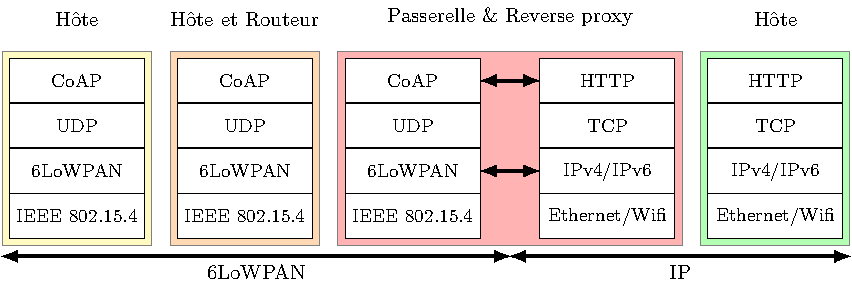
\includegraphics[width=\textwidth]{figures/network_stack_slides.pdf}
%   \end{figure}

%   \pnote{
%     - Propos général : les protocoles classiques sont adaptés aux réseaux de capteurs pour en faire des membres à part entières de l'Internet.
%   }

%   \pnote{
%     - IEEE 802.15.4: Couche Physique et MAC; topo maillé/étoilée; Faible cout
%   }
%   \pnote{
%     - 6LoWPAN: Compression IPv6
%   }
%   \pnote{
%     - RPL: Produit les routes montantes et descendantes;
%   }
%   \pnote{
%     - CoAP: Couche applicative; REST; UDP
%   }
% \end{frame}

% \begin{frame}{Zoom sur la passerelle}
%   \begin{figure}
%     \centering
%     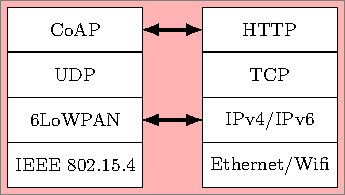
\includegraphics{figures/zoom_gateway_slides.pdf}
%   \end{figure}
%   \begin{block}{Protocoles}
%     \begin{itemize}
%       \item CoAP/HTTP: Traduction applicative
%       \item 6LoWPAN/IPv6: Encapsulation, compression des en-têtes
%     \end{itemize}
%   \end{block}
% \end{frame}

\begin{frame}{Moyen de contrôle de la passerelle}
  \begin{block}{Applicatif}
    \begin{itemize}
      \item Interception des messages applicatifs
    \end{itemize}
  \end{block}
  \begin{block}{Routage}
    \begin{itemize}
      \item Point central (Routage de bordure)
      \item Connaissance de la topologie (Dynamique ou statique)
      % \item Racine du DODAG (MP2P/P2MP)
      % \item Routeur de bordure (LBR)
    \end{itemize}
  \end{block}
  \begin{block}{Couche MAC}
    \begin{itemize}
      \item Connaît la couche MAC utilisée pour transmettre
    \end{itemize}
  \end{block}
  % \begin{block}{Couche réseau: 6LoWPAN}
  %   \begin{itemize}
  %     \item Compression IPv6
  %   \end{itemize}
  % \end{block}
  % \begin{block}{Couche physique et liaison: \ieee{}}
  %   \begin{itemize}
  %     \item PAN coordinator
  %   \end{itemize}
  % \end{block}
  \pnote{
    Ajouter que le proxy inverse sera détaillé par la suite.
  }
\end{frame}

% \begin{frame}{Passerelle intelligente}
%   \begin{figure}
%     \centering
%     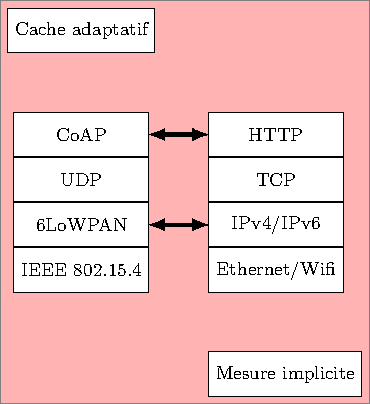
\includegraphics{figures/zoom_gateway_contrib_slides.pdf}
%   \end{figure}
% \end{frame}

% Annonce des contributions

\begin{frame}{Problématiques traitées dans la thèse}

  \begin{block}{Comment le connaître sans (trop) le solliciter ?}
    \begin{itemize}
      % \item Dimensionnement du réseau
      \item Surveillance matérielle et fonctionnelle %continue
      % \item Diagnostiquer ou anticiper des pannes
      \item Mesurer les grandeurs caractéristiques
    \end{itemize}
  \end{block}

  \begin{block}{Comment trouver le bon compromis ?}
    \begin{itemize}
      \item Économie de ressources
      \item Conserver un niveau de service suffisant
    \end{itemize}
  \end{block}

  \pnote{
    - Avoir une idée de trafic permet de dimensionner son réseau correctement (couverture, routeur intermédiaire)
    Ce qui apporte des gains de fiabilité et aide aux diagnostiques de problèmes.
  }
  \pnote{
    - Suivi de la disponibilité matérielle (un noeud mort) ou fonctionnelle (tout un étage est mort)
  }
  \pnote{
    - Prévoir l'évolution de métriques pour faire des interventions: Niveau de batterie, carte sd saturée
  }
  \pnote{---}
  \pnote{
    - Accorder les demandes des utilisateurs. Les rythmes de requetes importantes.
  }
  \pnote{
    - Servir une réponse depuis la passerelle va plus vite que depuis les noeuds
  }
\end{frame}


\begin{frame}\frametitle{Aperçu des contributions}


  \begin{figure}
    \centering
    %   \documentclass[crop,tikz]{standalone}% 'crop' is the default for v1.0, before it was 'preview'
% %\usetikzlibrary{...}% tikz package already loaded by 'tikz' option
% \usepackage[utf8]{inputenc}

% \usepackage{tikz}
% \usetikzlibrary{
%   arrows,
% automata,
% backgrounds,
% calc,
% decorations.pathreplacing,
% fit,
% petri,
% positioning,
% shadows,
% shapes,
% snakes,
% }


% % \begin{document}

  \begin{tikzpicture}%[scale = .8, every node/.style={scale = .8}]

%   % définition des styles
%   \tikzstyle{visible}=[draw, fill=blue!50]
%   \tikzstyle{hidden}=[ draw, fill=gray!20]
%   \tikzstyle{router}=[circle, draw, fill=orange!50,text=black]
%   \tikzstyle{child}=[circle, draw, fill=yellow!50,text=black]
%   \tikzstyle{root}=[circle, draw, fill=red!50,text=black]

  % les nœuds
  \node[draw,fill=red!50] (mesure) {\begin{tabular}{c}Mesure\\implicite\end{tabular}};
  \node[ left=of mesure] (traces) {\begin{tabular}{c}Traces\\ réseau\end{tabular}};
  \node[  right=of mesure] (estimation) {\begin{tabular}{c}Estimation\\ temps radio\end{tabular}};
%   \node[visible, below=of gw] (adapt) {Calcul des durées de validité optimales};


%   % Réseau contraint
%   \node[root] (1) at (-4, 0) {};
%   \node[router] (2) at (-5, 1) {};
%   \node[child] (3) at (-5, -1) {};
%   \node[child] (4) at (-6, 2) {};
%   \node[child] (5) at (-6, 0) {};

%   % \node[cloud, cloud puffs = 10, minimum width = 4cm, draw, fill = gray!10] (cloud) at (5,0) {Réseau local};
%   \node[draw] (cloud) at (5,0) {Réseau local};

%  \node [fit=(1) (2) (3) (4) (5), rounded corners, draw=black!50] (lln) {};
%  \node [below=.3 cm of lln] {LLN};

\path

	(traces) edge[->] (mesure)
	(mesure) edge[->] (estimation)

%   % Réseau contraint
%   (gw) edge[<->, thick] node [above] {$r_u$} (1)
%   (1) edge[<->] (2)
%   (1) edge[<->] (3)
%   (2) edge[<->] (4)
%   (2) edge[<->] (5)

%   % Réseau conventionnel
%   (gw.east) edge[<->, ultra thick] node [above] {$T_u$} (cloud)

%   % Cache
%   (gw) edge[->,very thick, bend left=10] node [midway,right] {$(\mathcal{T}, \mathcal{L})$} (adapt)
%   (adapt) edge[->,very thick, bend left=10] node [left] {$\mathcal{C}$} (gw)
  ;

  \end{tikzpicture}
  % \end{document}
  \end{figure}

  \begin{figure}
    \centering
    %   \documentclass[crop,tikz]{standalone}% 'crop' is the default for v1.0, before it was 'preview'
% %\usetikzlibrary{...}% tikz package already loaded by 'tikz' option
% \usepackage[utf8]{inputenc}

% \usepackage{tikz}
% \usetikzlibrary{
%   arrows,
% automata,
% backgrounds,
% calc,
% decorations.pathreplacing,
% fit,
% petri,
% positioning,
% shadows,
% shapes,
% snakes,
% }


% % \begin{document}

  \begin{tikzpicture}%[scale = .8, every node/.style={scale = .8}]

%   % définition des styles
%   \tikzstyle{visible}=[draw, fill=blue!50]
%   \tikzstyle{hidden}=[ draw, fill=gray!20]
%   \tikzstyle{router}=[circle, draw, fill=orange!50,text=black]
%   \tikzstyle{child}=[circle, draw, fill=yellow!50,text=black]
%   \tikzstyle{root}=[circle, draw, fill=red!50,text=black]

  % les nœuds
  \node[draw, fill=red!50,] (rpca) {\begin{tabular}{c}Cache\\adaptatif\end{tabular}};
  \node[ left=of rpca] (queries) {\begin{tabular}{c}Requetes\\ applicatives\end{tabular}};
  \node[draw, below=of rpca] (setup) {\begin{tabular}{c}Setup\end{tabular}};
  \node[ right=of rpca] (QUERIES) {\begin{tabular}{c}Requetes\\ applicatives\end{tabular}};

%   \node[visible, below=of gw] (adapt) {Calcul des durées de validité optimales};


%   % Réseau contraint
%   \node[root] (1) at (-4, 0) {};
%   \node[router] (2) at (-5, 1) {};
%   \node[child] (3) at (-5, -1) {};
%   \node[child] (4) at (-6, 2) {};
%   \node[child] (5) at (-6, 0) {};

%   % \node[cloud, cloud puffs = 10, minimum width = 4cm, draw, fill = gray!10] (cloud) at (5,0) {Réseau local};
%   \node[draw] (cloud) at (5,0) {Réseau local};

%  \node [fit=(1) (2) (3) (4) (5), rounded corners, draw=black!50] (lln) {};
%  \node [below=.3 cm of lln] {LLN};

\path
  (setup) edge[->] (rpca)

  (QUERIES) edge[->, ultra thick] (rpca)
  (queries) edge[<-, ultra thick, dashed] (rpca)

%   % Réseau contraint
%   (gw) edge[<->, thick] node [above] {$r_u$} (1)
%   (1) edge[<->] (2)
%   (1) edge[<->] (3)
%   (2) edge[<->] (4)
%   (2) edge[<->] (5)

%   % Réseau conventionnel
%   (gw.east) edge[<->, ultra thick] node [above] {$T_u$} (cloud)

%   % Cache
%   (gw) edge[->,very thick, bend left=10] node [midway,right] {$(\mathcal{T}, \mathcal{L})$} (adapt)
%   (adapt) edge[->,very thick, bend left=10] node [left] {$\mathcal{C}$} (gw)
  ;

  \end{tikzpicture}
  % \end{document}
  \end{figure}

  % \begin{alertblock}{Supervision passive}
  %   \begin{itemize}
  %     \item Observe le trafic au niveau du routeur de bordure
  %     \item Fournit une estimation de l'utilisation de la radio permettant de déduire une partie de la consommation énergétique
  %   \end{itemize}
  % \end{alertblock}

  % \begin{alertblock}{Reverse proxy adaptatif}
  %   \begin{itemize}
  %     \item Régule les temps de validité des réponses en cache au niveau de la passerelle
  %     \item Offre un compromis entre satisfaction des utilisateurs et économies d'énergie
  %   \end{itemize}
  % \end{alertblock}

  \pnote{
    Comment ajouter des services dans le dernier noeud non contraints qui est à la bordure du réseau standard ?
  }
  \pnote{
    - Dire que l'on a d'autres contributions mais que cette présentation se concentre sur celles présentées pour la passerelle.
  }

\end{frame}
